\section{Performance and Validation}\label{sec:results}

\subsection{Performance and Scaling}
We perform weak scaling tests for simulations of convection preceding ignition in a spherical, full-star sub-Chandrasekhar mass white dwarf.
The simulation setup remains the same as reported in Section 3 of \cite{MAESTRO_AMR} and originally used in \cite{MAESTRO_convection}, and thus we emphasize that these scaling tests are performed using meaningful, scientific calculations.
Here, we perform simulations using $256^3, 512^3, 768^3, 1024^3, 1280^3$, and $1536^3$ grid cells on a spatially uniform grid (no AMR).
We divide each simulation into $64^3$ grids, so this simulations contain between 64 grids ($256^3$) and 13,824 grids ($1536^3$).
These simulations were performed using the NERSC cori system on the Intel Xeon Phi (KNL) partition.
Each node contains 68 cores, each capable of supporting up to 4 hardware threads (i.e., a maximum of 272 hardware threads per node).
For these tests, we assign 4 MPI tasks to each node, and 16 OpenMP threads per MPI process.
Each MPI task is assigned to a single grid, so our tests use between 64 and 13,824 MPI processes (i.e., between 1,024 and 221,184 total OpenMP threads).
For $64^3$ grids we discovered that using more than 16 OpenMP threads did not decrease the wallclock time due to a lack of work available per grid; in principle one could use larger grids, fewer MPI processes, and more threads per MPI process to obtain a flatter weak scaling curve, however the overall wallclock time would increase except for extremely large numbers of MPI processes (beyond the range we tested here).
Thus, the more accurate measure of weak scaling is to consider the number of MPI processes, since the scaling plot would look virtually identical for larger thread counts.
Note that the largest simulation used roughly 36\% of the entire computational system.
%%%%%%%%%%%%%%%%%%%%%%%%%%%%%
\begin{figure}[htb]
\begin{center}
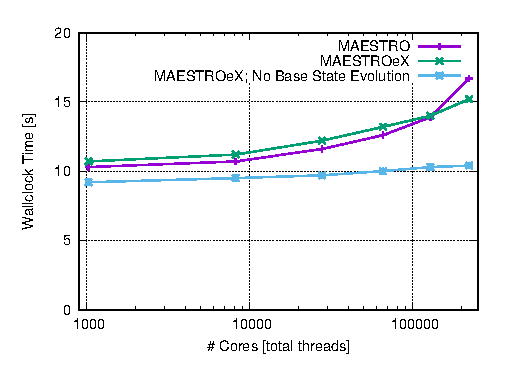
\includegraphics[width=2.75in]{./figs/MAESTRO_scaling1}
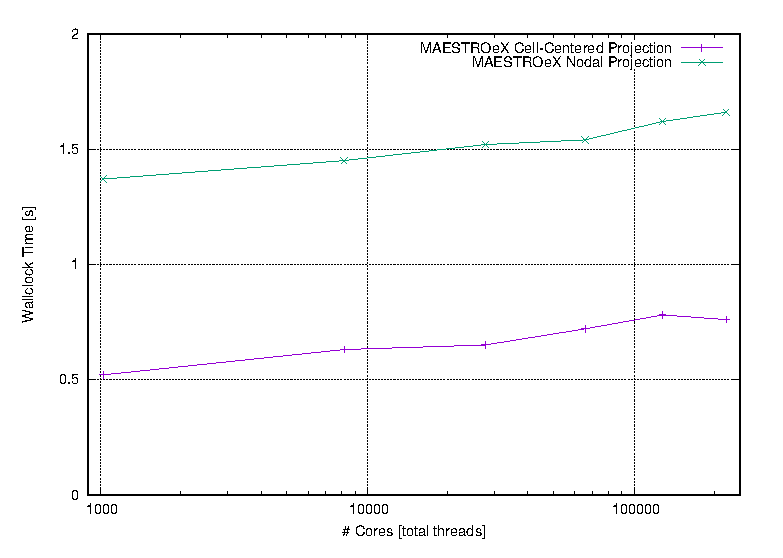
\includegraphics[width=2.75in]{./figs/MAESTRO_scaling2}
\caption{\label{fig:scaling} (Left) Weak scaling results for a spherical, full-star sub-Chandrasekhar mass white dwarf calculation using the original MAESTRO code, MAESTROeX, and MAESTROeX with base state evolution disabled.  Shown is the average wallclock time per time step.
(Right) Weak scaling results showing the average wallclock time per time step spent in the cell-centered and nodal linear solvers within a full time step of the aforementioned simulations.}
\end{center}
\end{figure}
%%%%%%%%%%%%%%%%%%%%%%%%%%%%%

In the left panel of Figure \ref{fig:scaling} we compare the wallclock time per time step as a function of total core count (in this case, the total number of OpenMP threads) for the original FBoxLib-based MAESTRO implementation to the AMReX MAESTROeX implementation.
These tests were performed using the original temporal integration strategy in \cite{MAESTRO_V}, noting that the new temporal integration with and without the irregular base state gives essentially the same results.
We also include a plot of MAESTROeX without base state evolution.
Comparing the original and new implementations, we see similar scaling results except for the largest simulation, where MAESTROeX performs better.
We see that the increase in wallclock time from the smallest to largest simulation is roughly 42\%.
We also note that without base state evolution, the code runs 14\% faster for small problems, and scale mush better
However, for the case without base state evolution, the overall runtime is faster and the increase in wallclock time from the smallest to largest simulation is roughly 13\%.
This is quite remarkable since there are 3 linear solver per time step (2 cell-centered Poisson solves used in the MAC projection, and a nodal Poisson solve used to compute the updated cell-centered velocities).
Contrary to our prior assumptions, the linear solves are not the primary scaling bottleneck in this code.
In the right panel of Figure \ref{fig:scaling}, we isolate the wallclock time required for these linear solves and see that (i) the linear solves only use 20-23\% of the total computational time, and (ii) the increase in the solver wallclock time from the smallest to largest simulation is only 28\%.
Further profiling reveals that the primary scaling bottleneck is the average operator.
The averaging operator requires binning the sum of Cartesian data onto one-dimensional arrays holding every possible mapping radius.
This amounts to at least 24,384 double precision values (for the $256^3$ simulation) up to 883,584 values (for the $1536^3$ simulation).
The averaging operator requires a global sum reduction over all processors, and the communication of this data is the primary scaling bottleneck.
For the simulation with base state evolution, this averaging operator is only called once per time step (as opposed to 14 times per time step when base state evolution is included).
The difference in total wallclock times with and without base state evolution is almost entirely due to the averaging.
Note that as expected, advection, reactions, and calls to the equation of state scale almost perfectly, since there is only a single parallel communication call to fill ghost cells.


\subsection{AMR Performance}

%%%%%%%%%%%%%%%%%%%%%%%%%%%%%
\begin{figure}[htb]
\begin{center}
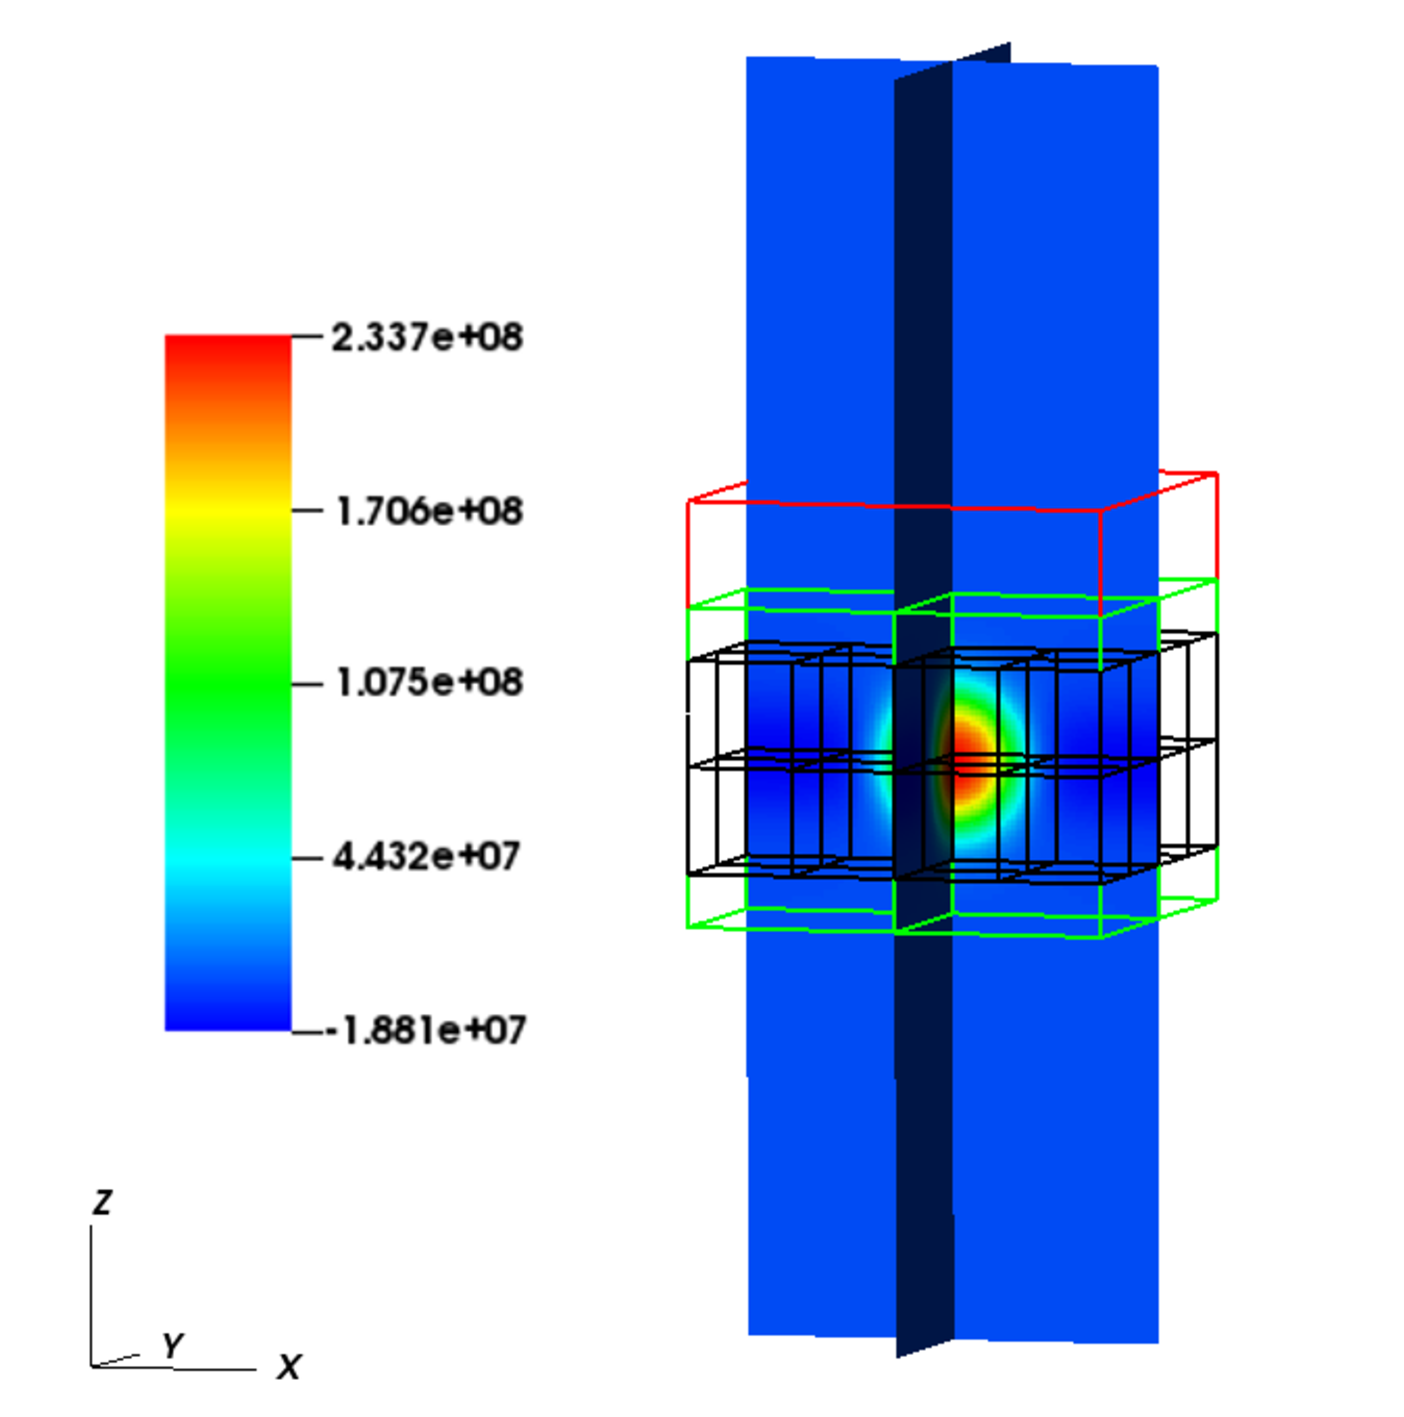
\includegraphics[width=2.75in]{./figs/reacting_bubble_amr} 
$\qquad$
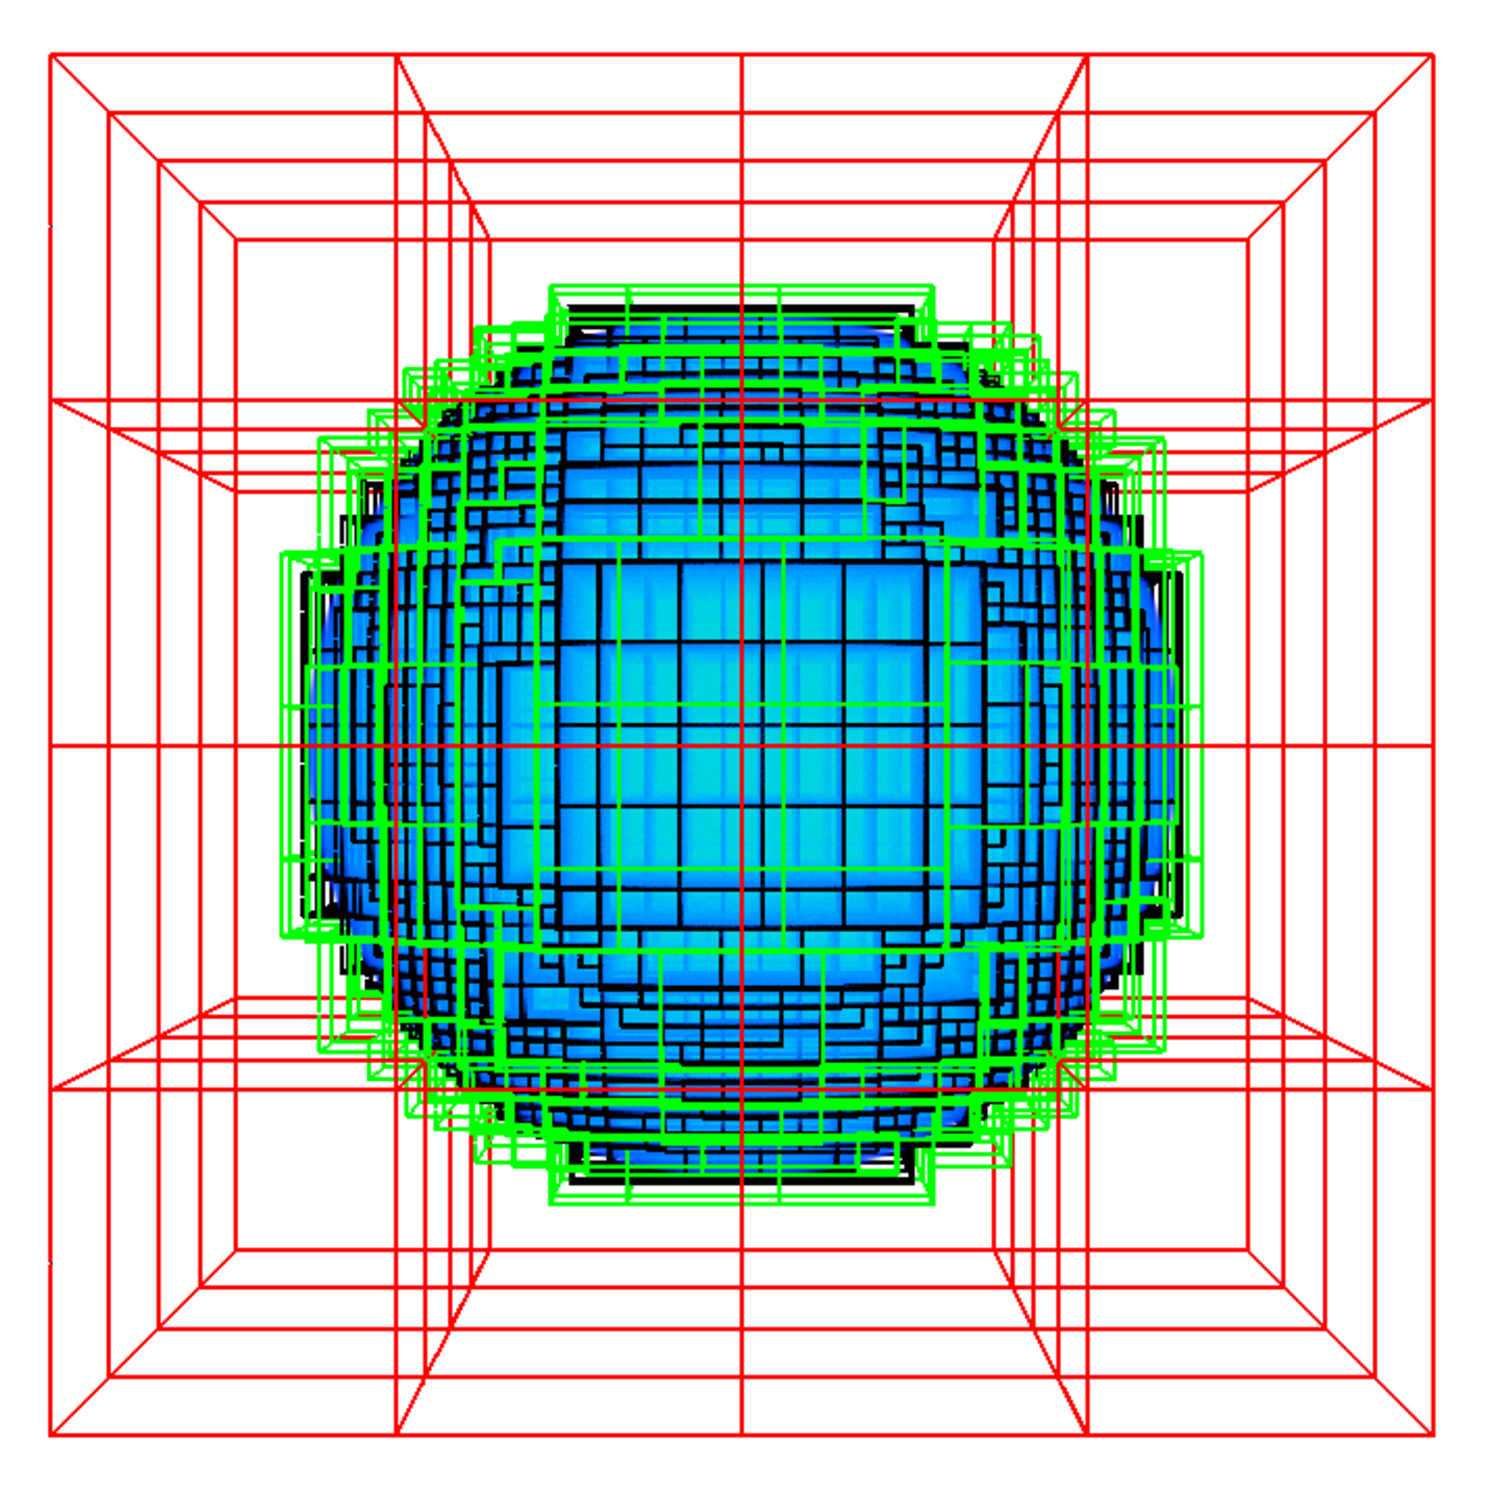
\includegraphics[width=2.75in]{./figs/wdconvect_amr_3grid}
\caption{\label{fig:amr_grids} Initial grid structures with two levels of refinement. 
         The red, green, and black lines represent grids of increasing refinement. 
         (Left) Profile of $T - \bar{T}$ for a hot bubble in a white dwarf environment.
         (Right) Region of star where $\rho\ge 10^5 \text{ g cm}^{-3}$ in a full white dwarf star simulation. }
\end{center}
\end{figure}
%%%%%%%%%%%%%%%%%%%%%%%%%%%%%

%%%%%%%%%%%%%%%%%%%%%%%%%%%%%
\begin{figure}[htb]
\begin{center}
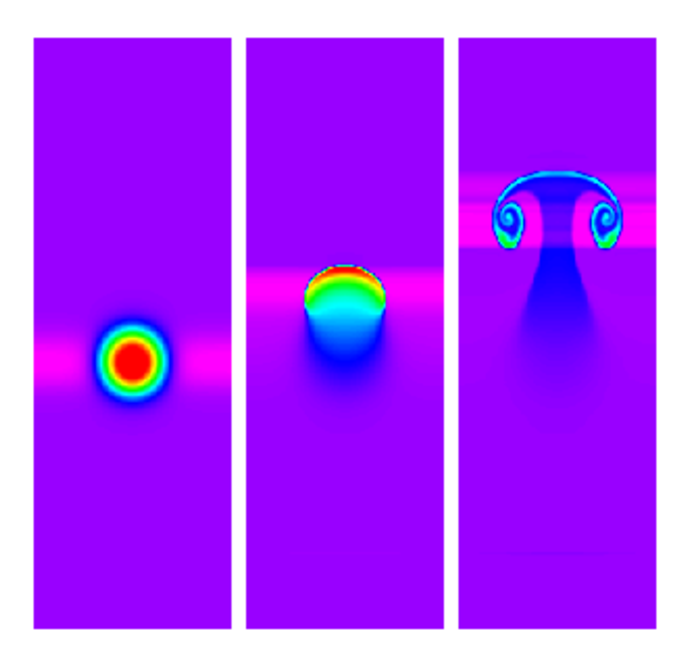
\includegraphics[width=2.75in]{./figs/reacting_bubble_result} 
$\qquad$
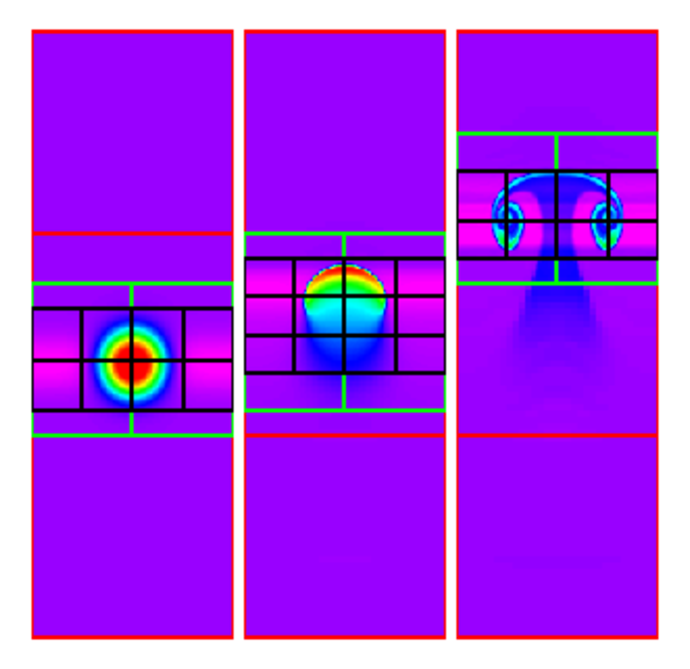
\includegraphics[width=2.75in]{./figs/reacting_bubble_amr_result}
\caption{\label{fig:bubble_results} Time-lapse cross-section of a hot bubble in a white dwarf environment at 
         $t = 0$, 1.25, and 2.5 s for (left) single-level simulation, and 
         (right) adaptive simulation at the same effective resolution.}
\end{center}
\end{figure}
%%%%%%%%%%%%%%%%%%%%%%%%%%%%%

Reacting bubble simulation at effective resolution of $128^2 \times 1024$ run on Cori Haswell with 48 processors took approximately 33.5 s per time step (averaged over 10 time steps) to run on single-level grid using either the original or new temporal algorithm, and only 3.7 s on adaptive grid with two levels of refinement. This 89\% decrease in runtime is mostly due to the fact that only 6.25\% of the cells (1,048,576 out of $128^2 \times 1024$ cells) are refined at the finest level for the AMR run. 




\subsection{White Dwarf Convection}

white dwarf convection runs with 3 algorithms (original, new temporal, new temporal + variable-spaced base state)

%%%%%%%%%%%%%%%%%%%%%%%%%%%%%
\begin{figure}[htb]
\begin{center}
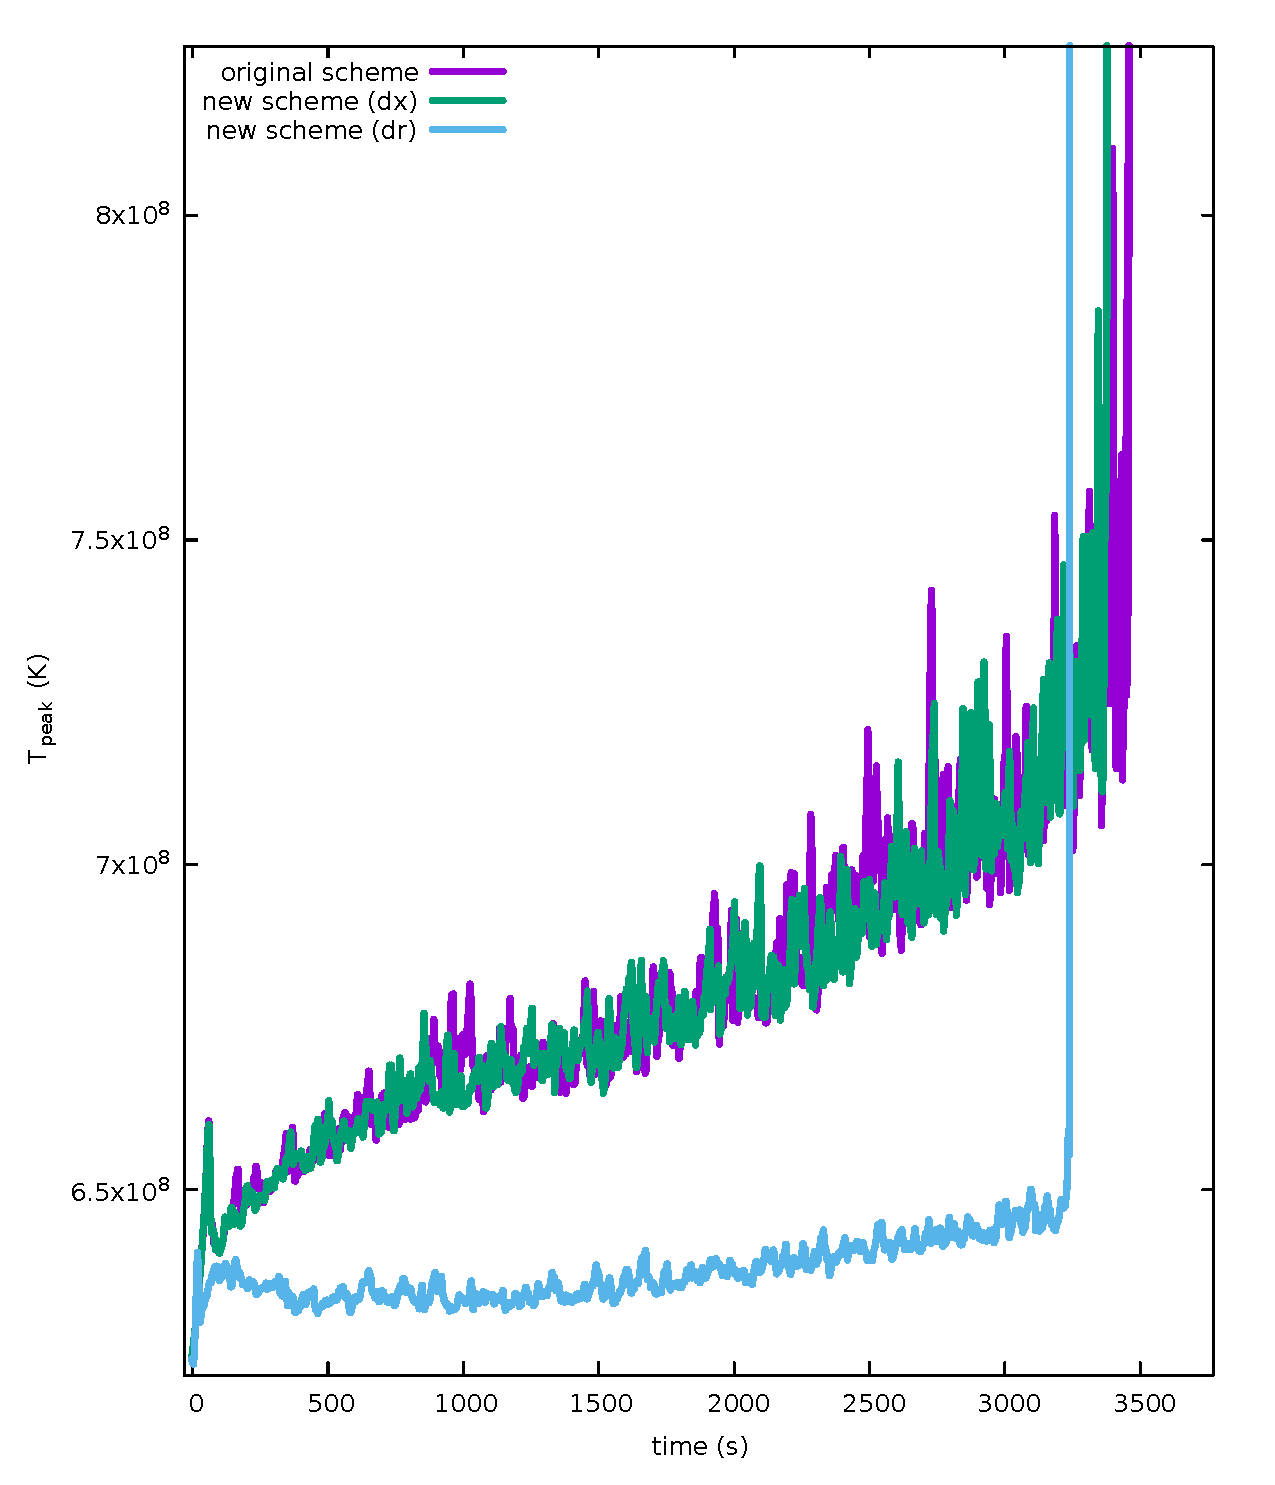
\includegraphics[width=2.75in]{./figs/wdconvect_128_maxT}  \hspace{0.5in}
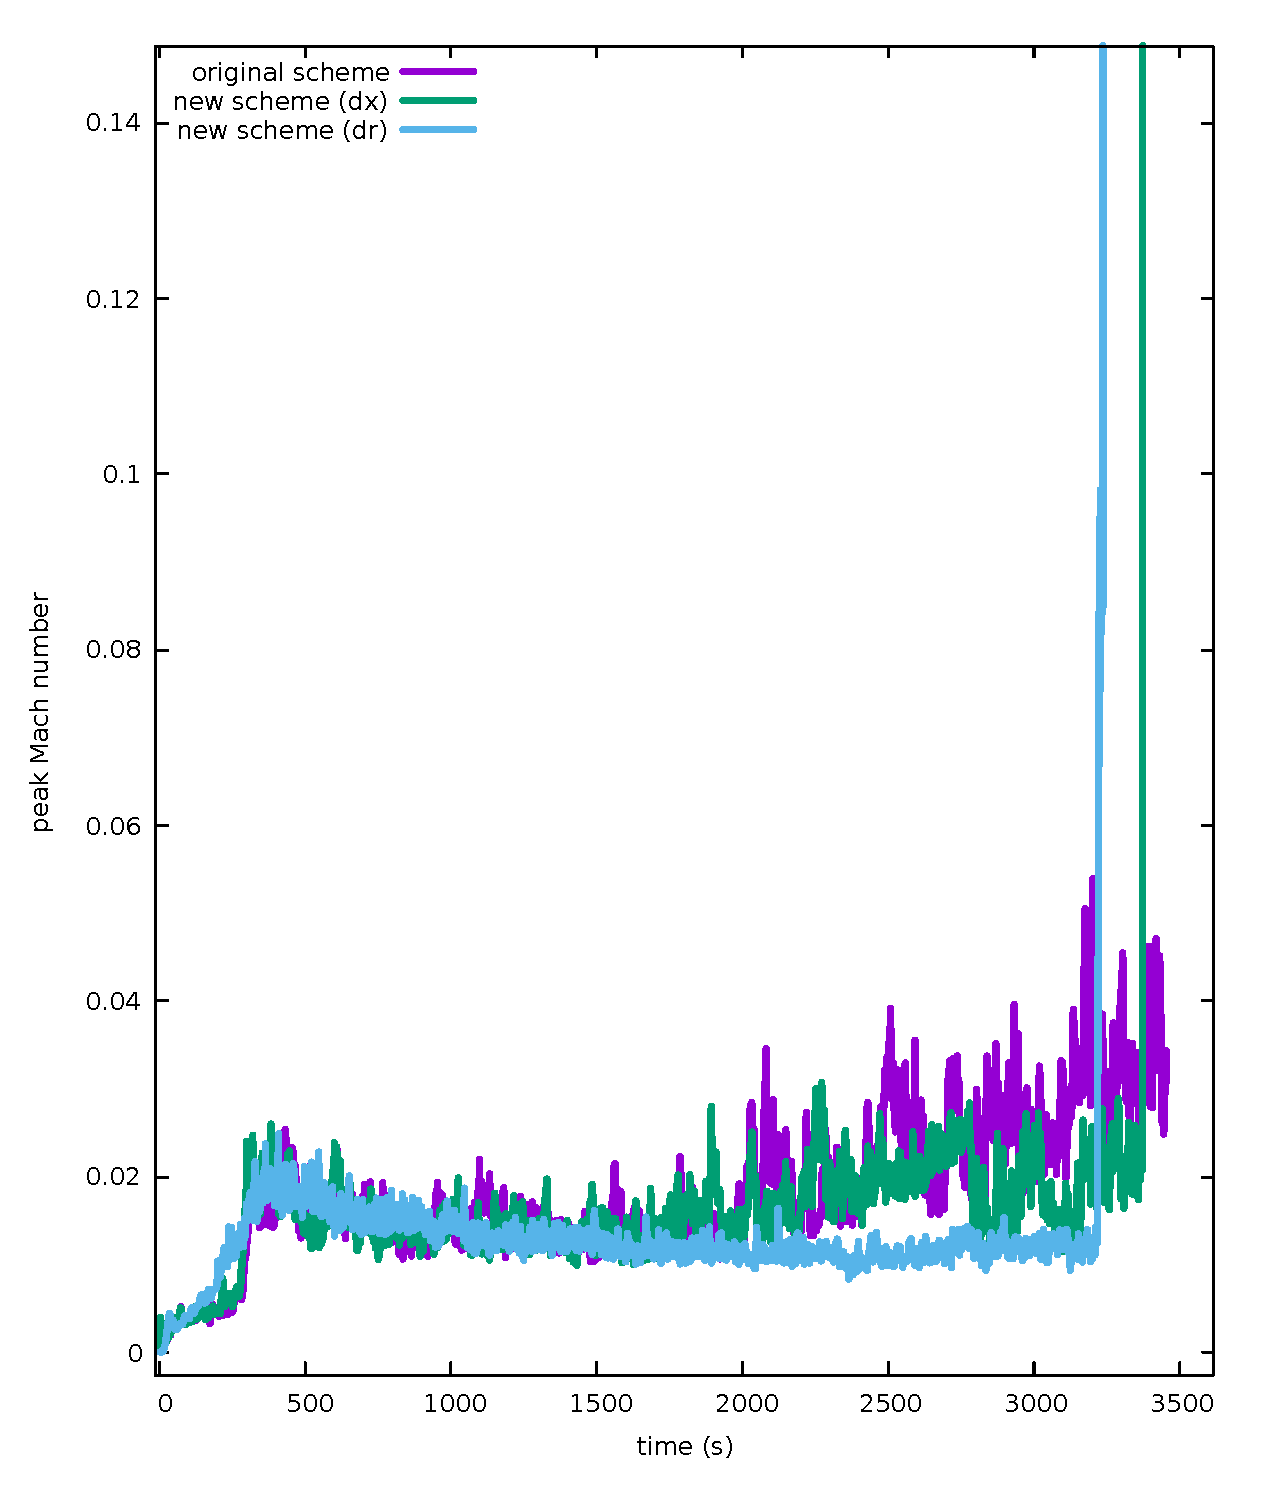
\includegraphics[width=2.75in]{./figs/wdconvect_128_maxMach}
\caption{\label{fig:wdconvect_128_maxval} (left) Peak temperature, $T_{\text{peak}}$, and (right) peak Mach number 
         in a white dwarf until time of ignition at resolution of $128^3$ for three different MAESTROeX algorithms.}
\end{center}
\end{figure}
%%%%%%%%%%%%%%%%%%%%%%%%%%%%%

%%%%%%%%%%%%%%%%%%%%%%%%%%%%%
\begin{figure}[hbt]
\begin{center}
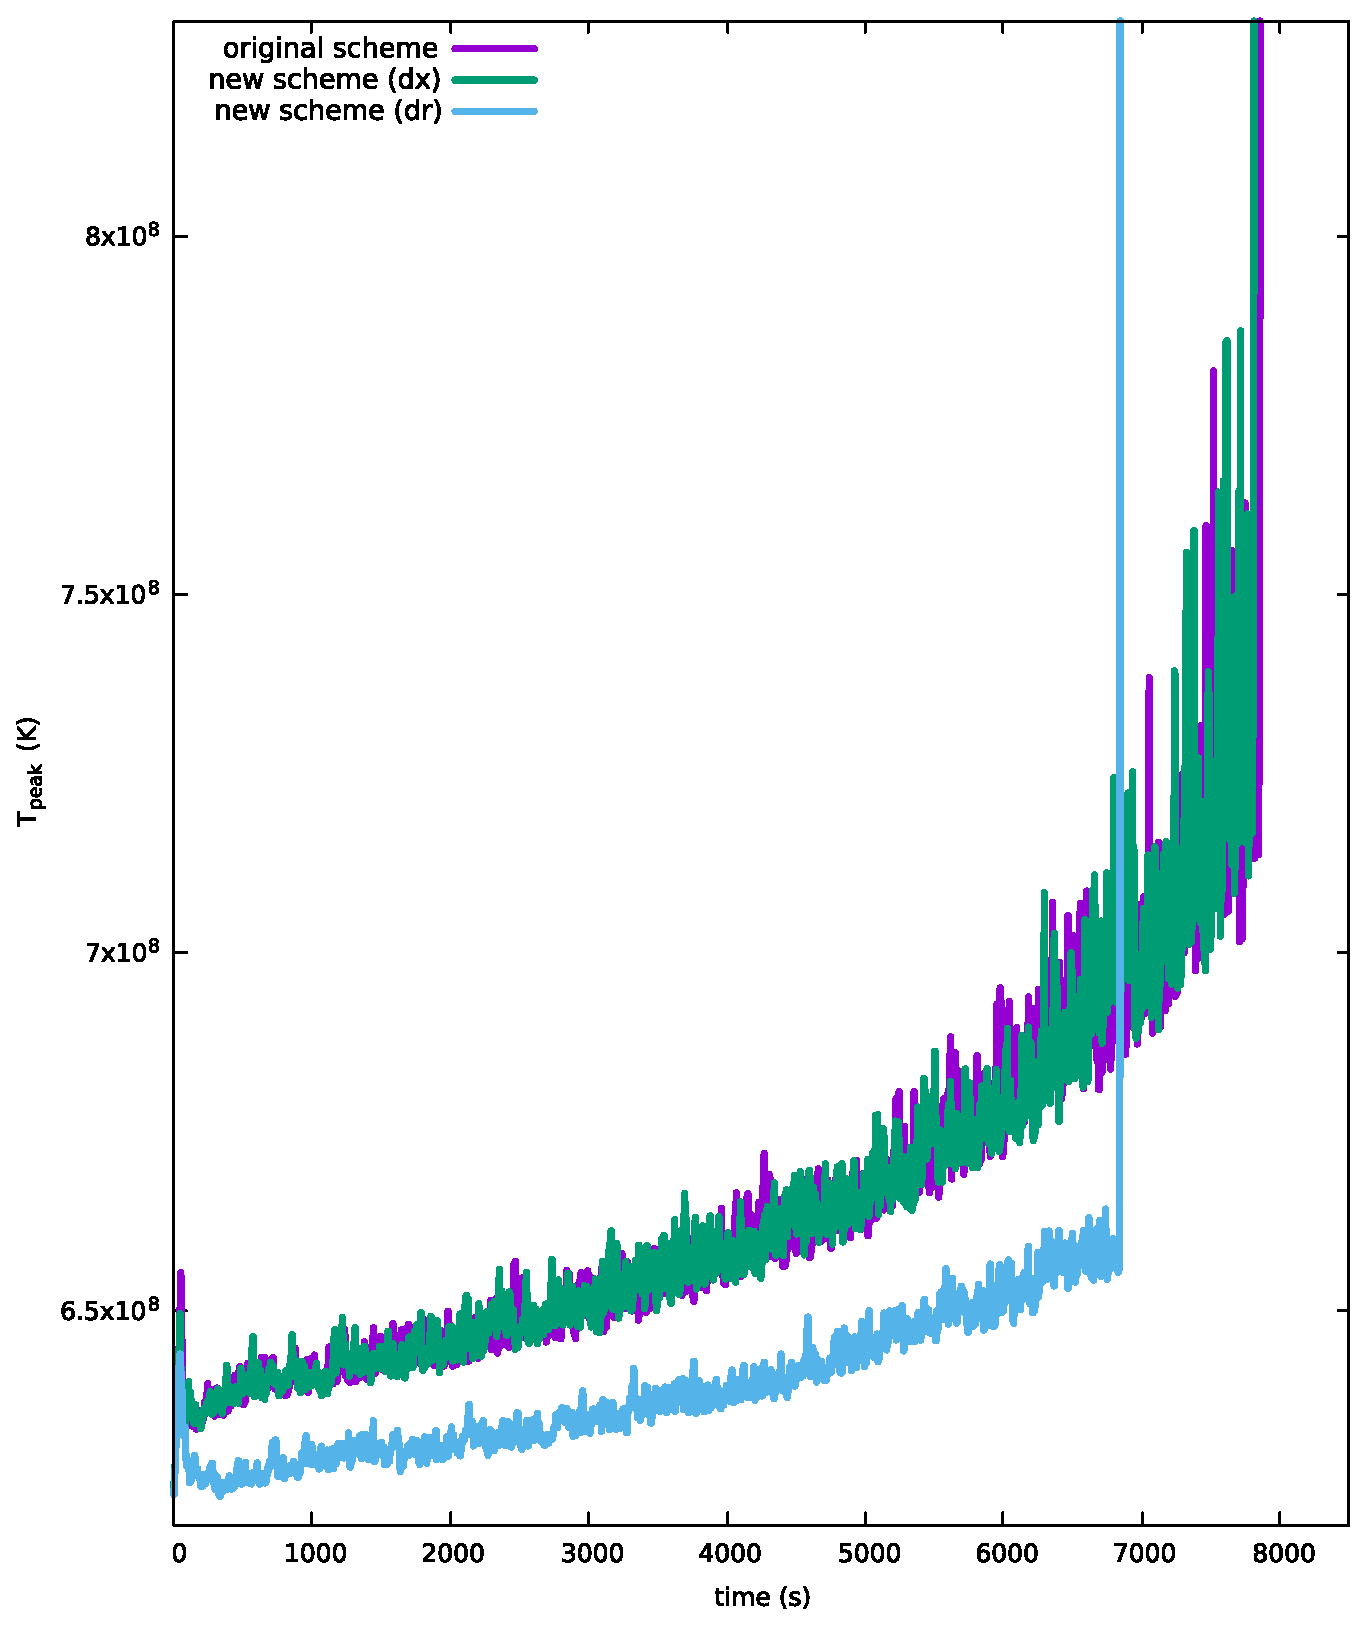
\includegraphics[width=2.7in]{./figs/wdconvect_256_maxT}  \hspace{0.5in}
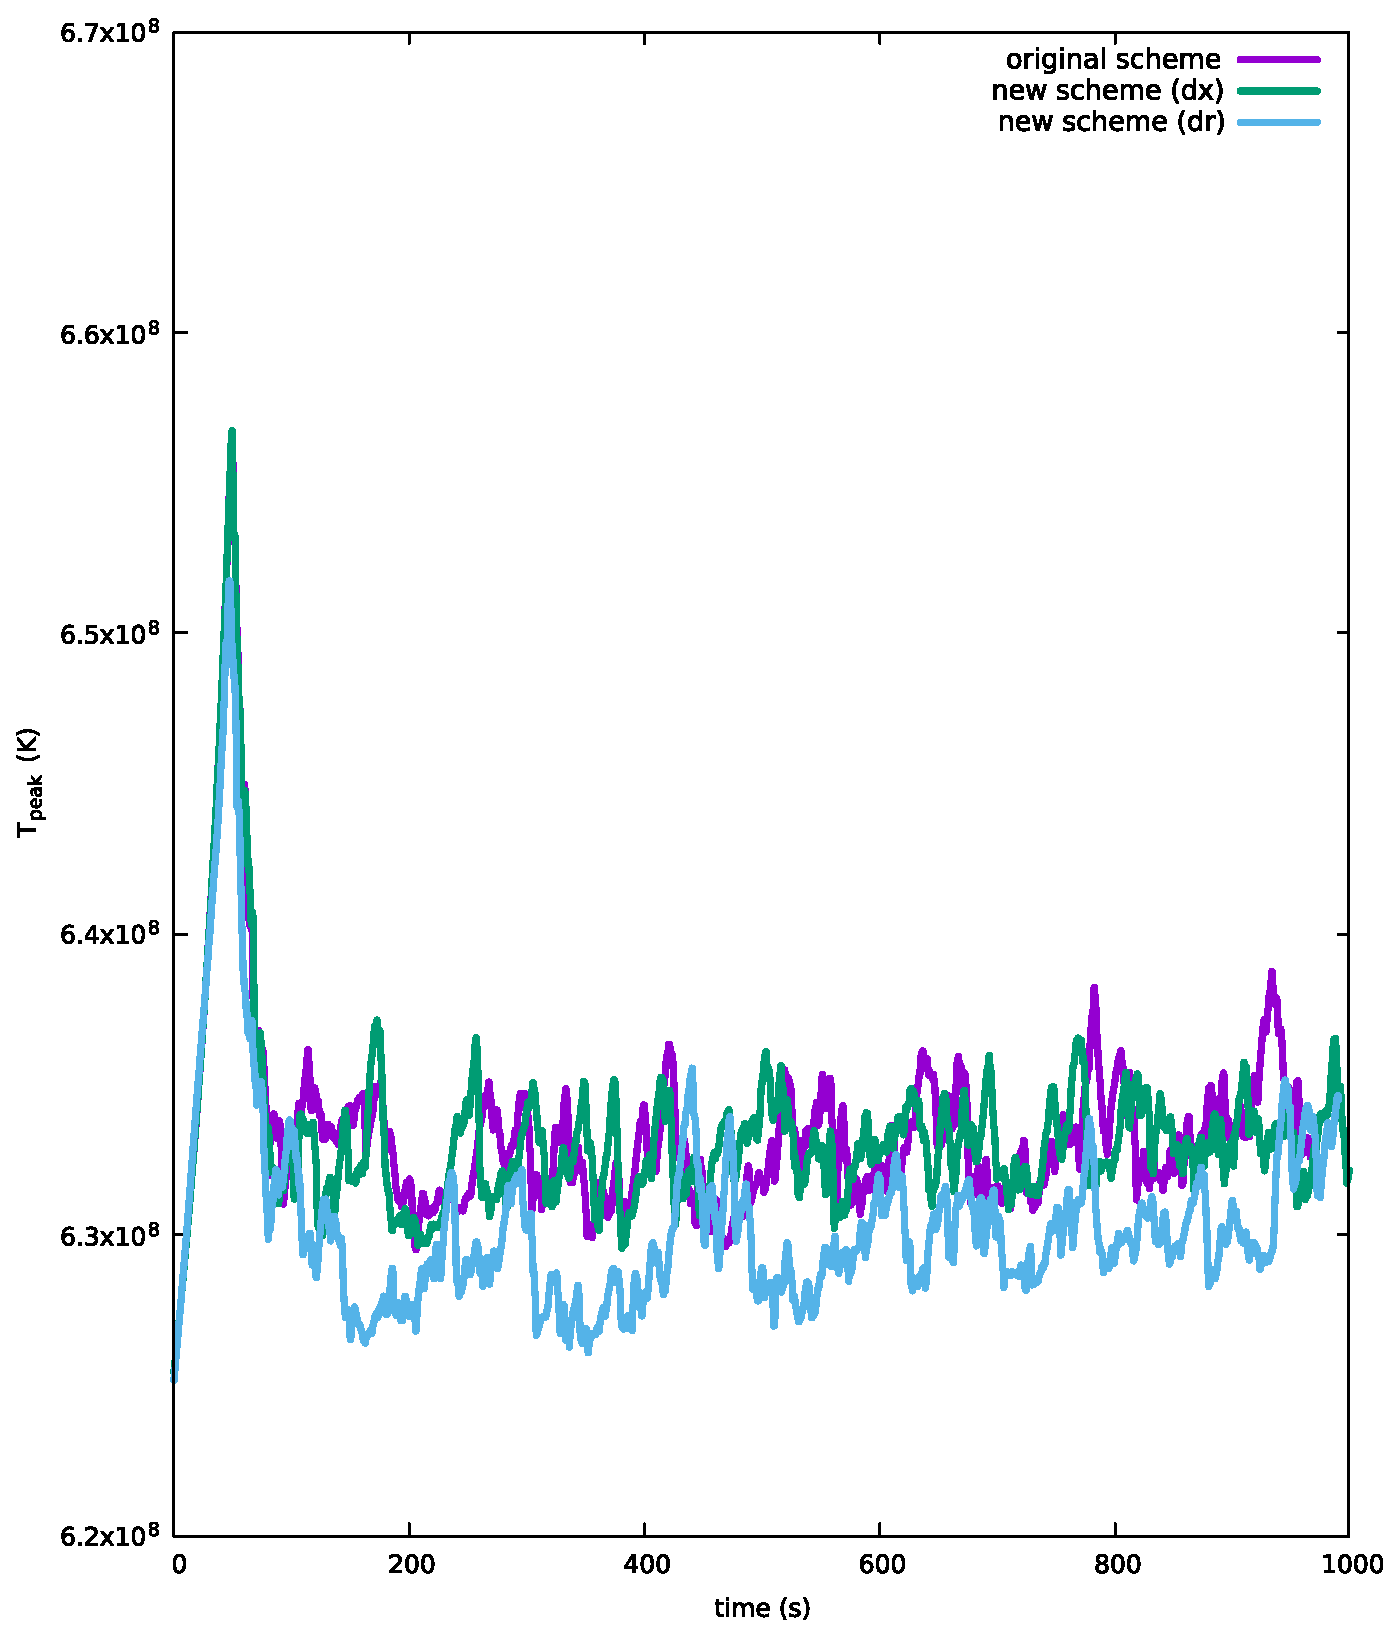
\includegraphics[width=2.75in]{./figs/wdconvect_512_maxT}
\caption{\label{fig:wdconvect_Tmax} Peak temperature, $T_{\text{peak}}$  in a white dwarf at 
         (left) resolution of $256^3$ until time of ignition and (right) resolution of $512^3$ until $t=1000$ 
         for three different MAESTROeX algorithms. Note that the variable-spaced (d$r$) solution agrees better 
         with the evenly-spaced solution as the resolution increases.}
\end{center}
\end{figure}
%%%%%%%%%%%%%%%%%%%%%%%%%%%%%


\subsection{AMR}

%%%%%%%%%%%%%%%%%%%%%%%%%%%%%
\begin{figure}[htb]
\begin{center}
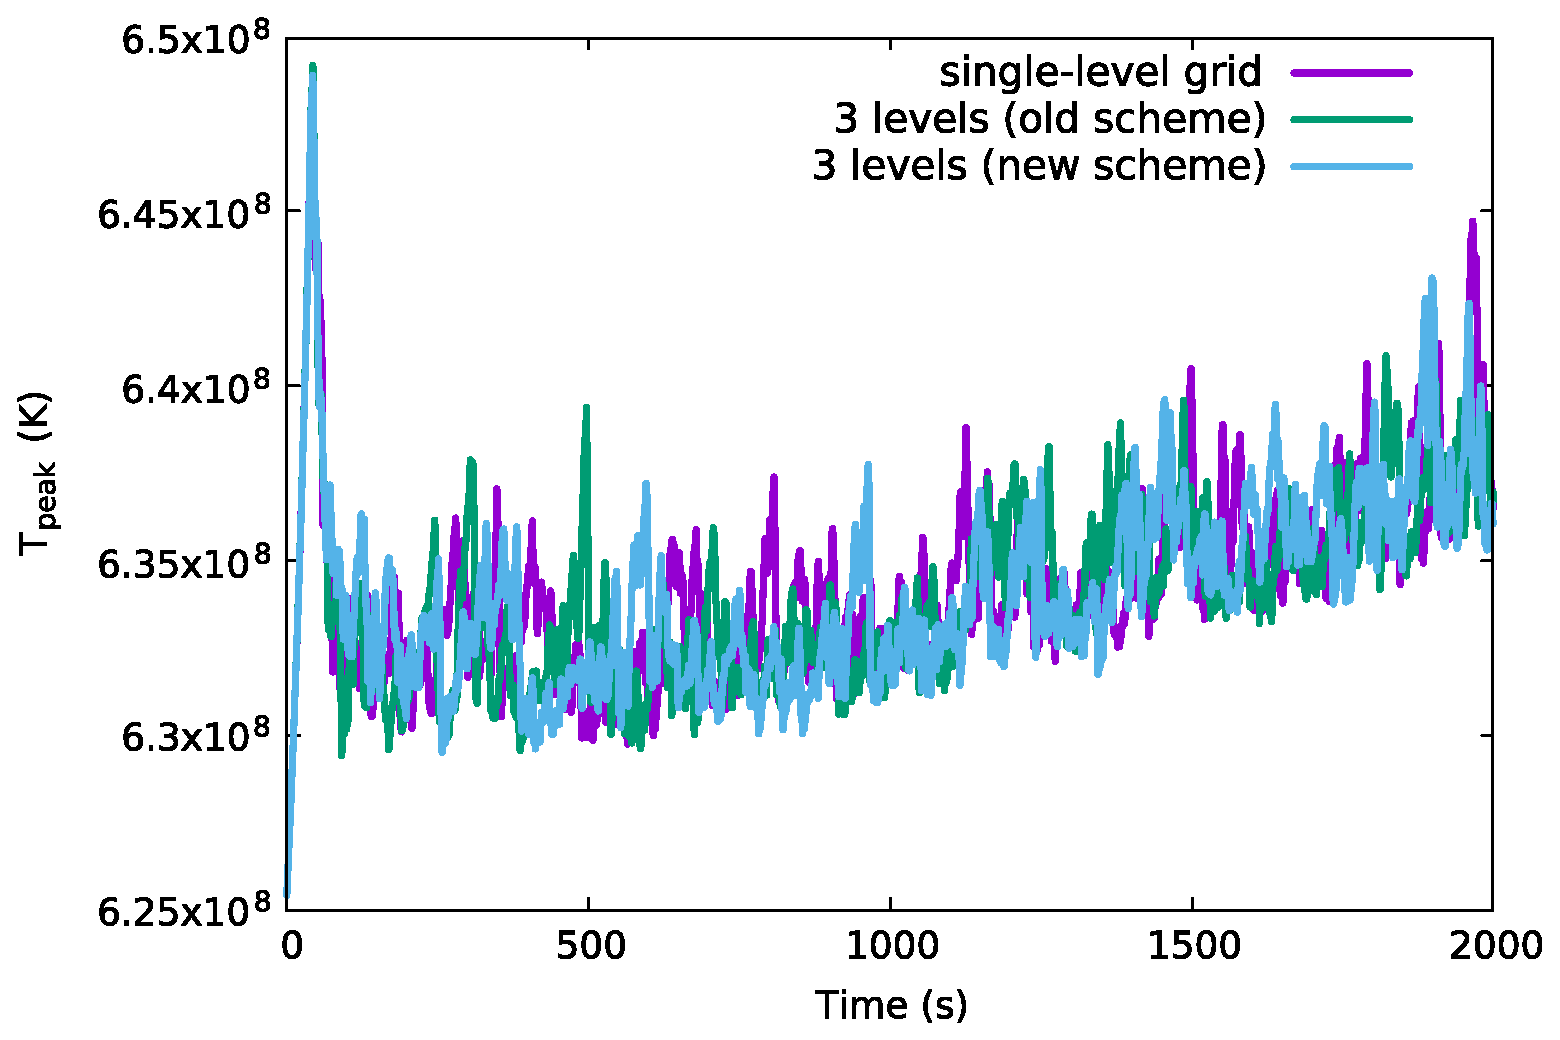
\includegraphics[width=4.0in]{./figs/wdconvect_amr_Tmax} 
\caption{\label{fig:wdconvect_amr_Tmax} Peak temperature, $T_{\text{peak}}$, in a white dwarf from $t=0$ to $400$ s 
         for grids with effective resolution of $512^3$. We can see that the adaptive grids with two levels of 
         refinement give very similar solution trends compared to the single-level grid.}
\end{center}
\end{figure}
%%%%%%%%%%%%%%%%%%%%%%%%%%%%%

Full white dwarf star simulation at effective resolution of $512^3$ on Cori KNL with 512 processors and 16 threads took 26.01 s per time step (averaged over 10 time steps) using the original temporal scheme, and 22.66 s using the new scheme. On an adaptive grid with two levels of refinement, 8.9\% of the cells (1,493,504 out of $256^3$ cells) are refined at the first level and 5.3\% (7,176,192 out of $512^3$ cells) at the second. The simulation took 11.55 s and 12.48 s using the orginial and new temporal schemes, respectively. 
